%https://kvant.ras.ru/pdf/2014/2014-56.pdf
% \documentclass[twoside]{article}
% \usepackage[utf8]{inputenc} % Включаем поддержку UTF8
% \usepackage{multicol}
% \usepackage[russian]{babel}
% \usepackage{ mathrsfs }% для красивой буквы E
% \usepackage{graphicx}
% \usepackage[a4paper,top=2cm,bottom=2cm,left=1cm,right=1cm,marginparwidth=1.75cm]{geometry}
% \usepackage{wrapfig}
% \usepackage[fontsize=9pt]{fontsize}
% \setcounter{page}{84}
% \setlength{\parindent}{0cm}


% \setcounter{page}{84}

% \makeatletter
% \def\ps@myPS{%

%     \def\@evenhead{
%     \thepage\\
%     \textbf{КВАНT} 2014/№5-6\\
%     }
    
%     \def\@oddhead{
%     \\
%     \textbf{КВАНT} 2014/№5-6\\
%     \thepage
%     }
    
%     \def\@evenfoot{}
    
%     \def\@oddfoot{}
%     }
% \makeatother

% \thispagestyle{myPS}
\begin{multicols}{2}
4. Работа силы трения на каждом маленьком участке
${\Delta}s$
равна
${\Delta}A = -F_{\mbox{тр}}{\Delta}s$
, а сама сила трения равна\\
\[ F_{\mbox{тр}} = {\mu}mg(cos {\alpha} - \frac{v^2}{Rg}),\]
где R – радиус кривизны траектории. Поэтому в общем случае, для того чтобы работа силы трения при подъеме была
равна работе силы трения при спуске, необходимо, чтобы
скорости тела на одном и том же участке при спуске и при
подъеме были одинаковыми. Впрочем, всех этих сложностей
можно избежать, если представлять горку в таких задачах
прямой ($R = \infty$) с небольшим покрытым льдом ($\mu = 0$) переходным участком от наклонной части траектории к горизонтальной.

{\centering\textbf{\mbox{Задачи}}\par}

5. На рисунке 8 приводится таблица «Физического судоку»,
заполненная с использованием неизвестной $A_x$.
Коэффици-

{\centering
\begin{tabular}{| c | c | c | c |}
    \hline
     & $Q=$ & ${\Delta}U+$ & $A_x$ \\ 
    \hline
    1-2 & $0$ & $-\frac{3}{2}A_1$ & $\frac{3}{2}A_1$\\  
    \hline
    2-3 & $-A_x$ & $0$ & $-A_x$\\
    \hline
    3-1 & $\frac{5}{2}A_1$ & $\frac{3}{2}A_1$ & $A_1$\\
    \hline
    ${\sum}$ & & 0 & $\frac{5}{2}A_1 - A_x$\\
    \hline
\end{tabular}
\par}
\hspace{2.1cm}\textit{Рис. 8}

ент полезного действия связывает клетки таблицы следующим
образом:
\[\eta = \frac{A_{\mbox{общ}}}{Q_{\mbox{общ}}} = \frac{(5/2)A_1-A_x}{(5/2)A_1}\]
откуда следует ответ:
\[ A_x = (1-\eta)*\frac{5}{2}A_1=1200\mbox{ Дж} \]
7. На рисунке 9 приводится заполненная таблица. Ответ имеет вид
\[ A = 2mgh = \frac{mv^2}{2} = 460\mbox{ Дж} \]
{\centering
    \begin{tabular}{ | c | c | c | c | }
        \hline
         & $A_{\mbox{пуст}}$+ & $A_{\mbox{тр}}=$ & ${\Delta}E$ \\
        \hline
        1-2 & 0 & -210 & -210 \\
        \hline
        2-1 & 460 & -210 & 250 \\
        \hline
    \end{tabular}
\par}
\hspace{2.1cm}\textit{Рис. 9}

\begin{center}
    \textbf{КОЛЕБАТЕЛЬНЫЙ КОНТУР И ЗАКОНЫ СОХРАНЕНИЯ}
\end{center}

\textbf{1.} $q = 2\mbox{ нКл}$.
\textbf{2. }$L = (\frac{q}{I_0(C_1-C_2)})^2C_1$.
\textbf{3. }$I_{1m}=\frac{2LI_m}{L+L_1}$.

\textbf{4. }$q_m=\sqrt{q^2+\frac{2LCI^2}{3}}$.
\textbf{5. }$Q = 115\mbox{ мДж}$.
\textbf{6. }$I_m = 7\mathscr{E}\sqrt{\frac{C}{L}}$.

\textbf{7. }$Q = \frac{L_1L_2I_m^2}{2(L_1+L_2)}$.
\textbf{8. }$Q = \frac{\mathscr{E}^2}{2}(C+\frac{L}{R^2})$.
\textbf{9. }$Q = \frac{CU_0^2}{2}+\frac{L_1L_2I_0^2}{2(L_1+L_2)}$.

\textbf{10. }1) $I = \frac{\mathscr{E}}{R}$; 2) $U_m=\frac{\mathscr{E}}{R}\sqrt{\frac{L_1L_2}{C(L_1+L_2)}}$.

\columnbreak

\begin{center}
    \textbf{ЗАКЛЮЧИТЕЛЬНЫЙ ЭТАП XL ВСЕРОССИЙСКОЙ ОЛИМПИАДЫ ШКОЛЬНИКОВ ПО МАТЕМАТИКЕ}
    
    \textit{9 класс}
\end{center}

\textbf{1.} Пусть ни одно из чисел не делится на 3. Тогда каждое число дает остаток 1 или 2 при делении на 3. Но числа, дающие
одинаковые ненулевые остатки при делении на 3, не могут отличаться на 1 или на 2; не могут они отличаться и в два раза.
Значит, соседние числа дают различные остатки при делении
на 3, т.е. остатки 1 и 2 чередуются. Но тогда общее количество чисел должно быть четным, что не так. Противоречие

\textbf{2.} Два.
Заметим, что никакие два квадрата натуральных чисел не отличаются на 1, ибо $x^2-y^2=(x-y)(x+y)$, где вторая скобка больше единицы. Значит, числа $a(a+2)=(a+1)^2-1$ и $b(b+2)=(b+1)^2-1$ квадратами не являются. Более того,
числа $ab$ и $a(b+2)$ не могут одновременно являться квадратами, иначе их произведение $a^2b(B+2)$ также было бы квадратом, а тогда и число $b(b+2)$ – тоже. Аналогично, из чисел $(a+2)b$ и $(a+2)(b+2)$ максимум одно может быть квадратом. Итого, квадратов на доске не больше двух. Два квадрата могут получиться, например, при $а = 2$ и
$b = 16$: тогда $(a(b+2)=6^2$ и $(a+2)b = 8^2$.

\textbf{3.} $n-2$ при четных $n$, $n-3$ при нечетных $n$. Мы будем пользоваться следующей известной леммой.

\textbf{Лемма.} \textit{В выпуклом n-угольнике нельзя провести более $n - 3$
диагоналей, не имеющих общих внутренних точек.}

Сначала докажем индукцией по $n$, что количество хороших
диагоналей не превосходит $n - 2$, если $n$ четно, и $n - 3$, если $n$ нечетно. При этом мы будем считать, что отрезок является 2-угольником без диагоналей. При $n=2$, 3 утверждение очевидно. Пусть $n \geq 4$ ; обозначим наш многоугольник через $P=A_1A_2{\ldots}A_n$ .

Если никакие две хорошие диагонали не пересекаются, то по
лемме их количество не превосходит $n - 3$. Пусть теперь найдутся две пересекающихся хорошие диагонали $A_iA_k$ и $A_jA_l$ $(i<j<k<l)$.
\begin{wrapfigure}{r}{0.2\textwidth}
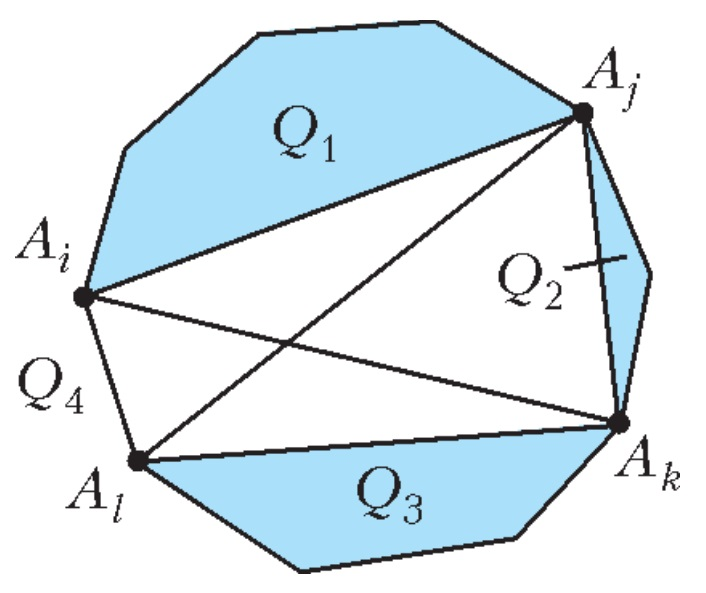
\includegraphics[width=0.2\textwidth]{img.jpg}\\
Рис. 10
\end{wrapfigure}
Тогда каждая из них не пересекается с другими
проведенными диагоналями. Выбросим $A_iA_k$ и $A_jA_l$ из рассмотрения. Каждая оставшаяся проведенная диагональ $d$ является диагональю или стороной ровно в одном из многоугольников $Q_1=A_i{\ldots}A_j , Q_2 = A_j{\ldots}A_k , Q_3 = A_k{\ldots}A_l$ или $Q_4 = A_l{\ldots}A_nA_1{\ldots}A_i$(рис.10). При этом если $d$ является стороной одного из них, то она не может пересекаться с другими диагоналями (и не является хорошей).

Пусть $n$ четно. По предположению индукции, среди всех диагоналей, попавших в какой-то многоугольник $Q_s$
, хороших не больше, чем количество вершин в нем, уменьшенное на $2$.
Значит, общее количество хороших диагоналей в $P$ не превосходит
\[ 2+(j-i-1)+(k-j-1)+(l-k-1)+(n-l+i-1)=n-2 , ( * )\]
что и требовалось.

При нечетном $n$ сумма количеств вершин в многоугольниках $Q_1$ , $Q_2$ , $Q_3$ , $Q4$ равна нечетному числу $n + 4$; значит, число вершин в одном из них нечетно. А тогда соответствующее
слагаемое в сумме ( * ) уменьшится на 1, и мы получим, что
общее число хороших диагоналей не превосходит $n - 3$. Переход индукции завершен

Осталось привести примеры, показывающие точность оценки.
При четном $n$ достаточно провести в многоугольнике $A_1{\ldots}A_n$
\end{multicols}
\clearpage
\LaTeX